% ============================================================
% TD : Équations différentielles du premier ordre (version 2.0)
% Pôle Formation UIMM - CVDL - BTS Industriel - S. JAUBERT
% Remplace TD_EDL1_MOD06_app (février 2026).
% Corrigé enseignant : MOD06_EDL1_TD_Corrige_v2_0
% Compilation : pdflatex, deux passes (nombre total de pages).
% Version 2.0, révision du 07/10/2026 : partie C étendue à 9 exercices (séparables, homogène, Bernoulli, Euler).
% ============================================================
\documentclass[a4paper,11pt]{article}
\usepackage[utf8]{inputenc}
\usepackage[T1]{fontenc}
% babel-french absent sur certains postes : chargement conditionnel
\IfFileExists{french.ldf}{\usepackage[french]{babel}}{}
\usepackage{helvet}
\renewcommand{\familydefault}{\sfdefault}
\renewcommand{\ttdefault}{lmtt}
\usepackage[top=2cm, bottom=3cm, left=2cm, right=2cm, headheight=14pt, footskip=1.6cm]{geometry}
\usepackage{amsmath,amssymb}
\usepackage{graphicx}
\usepackage[dvipsnames,table]{xcolor}
\usepackage{tikz}
\usetikzlibrary{arrows.meta, patterns, calc}
\usepackage{pgfplots}
\pgfplotsset{compat=1.18}
\usepackage[european]{circuitikz}
\usepackage[most]{tcolorbox}
\usepackage{fancyhdr}
\usepackage{enumitem}
\usepackage{array,tabularx,needspace}
\usepackage{lastpage}
\usepackage{listings}
\usepackage{hyperref}

% ----- Charte UIMM -----
\definecolor{uimmblue}{HTML}{005C85}
\definecolor{uimmred}{HTML}{D31326}
\definecolor{uimmlightblue}{HTML}{E8F1F8}
\definecolor{uimmgray}{HTML}{333333}
\definecolor{uimmlightgray}{HTML}{F5F5F5}
\hypersetup{colorlinks=true, linkcolor=uimmblue, urlcolor=uimmblue}
\setlength{\parindent}{0pt}
\setlength{\parskip}{3pt}

\setlist[enumerate,1]{label={\color{uimmblue}\textbf{\arabic*.}}, leftmargin=*, itemsep=2pt}
\setlist[enumerate,2]{label=\alph*), itemsep=1pt}
\setlist[itemize,1]{label={\color{uimmblue}\textbullet}}

% ----- Code Python copiable depuis le PDF -----
% Police vectorielle + espaces réels peints dans la couleur du fond :
% l'indentation est conservée au copier-coller dans la plupart des lecteurs.
\input{glyphtounicode}
\pdfglyphtounicode{uni2423}{0020}
\pdfgentounicode=1
\lstdefinestyle{uimmpython}{
  basicstyle=\ttfamily\small,
  keywordstyle=\color{uimmblue}\bfseries,
  commentstyle=\color{green!50!black}\itshape,
  stringstyle=\color{uimmred},
  numbers=none, columns=fullflexible, keepspaces=true, upquote=true,
  showspaces=true, showstringspaces=false, breaklines=false,
  frame=single, rulecolor=\color{uimmblue}, backgroundcolor=\color{uimmlightgray},
  xleftmargin=4pt, xrightmargin=4pt, aboveskip=6pt, belowskip=6pt,
  language=Python, extendedchars=true, inputencoding=utf8,
  literate={é}{{\'e}}1 {è}{{\`e}}1 {à}{{\`a}}1 {°}{{\textdegree}}1 {²}{{\textsuperscript{2}}}1 {ç}{{\c c}}1 {ê}{{\^e}}1 {î}{{\^\i}}1
}
\makeatletter
\def\lst@visiblespace{\textcolor{uimmlightgray}{\char32}}
\makeatother

% ----- En-tête et pied de page (modèle PR3) -----
\pagestyle{fancy}
\fancyhf{}
\renewcommand{\headrulewidth}{0pt}
\fancyfoot[C]{\small\renewcommand{\arraystretch}{1.3}%
\begin{tabularx}{\textwidth}{|>{\centering\arraybackslash\itshape}X|>{\centering\arraybackslash}p{1.8cm}|>{\centering\arraybackslash}p{3.6cm}|>{\centering\arraybackslash}p{1.9cm}|}
\hline
BTS Industriel -- MOD06 Équations différentielles -- [S01] & {\scriptsize\itshape Auteur :}\newline SJ & MAJ du 07/10/2026\newline{\color{uimmblue}Version 2.0} & Page :\newline \thepage/\pageref*{LastPage}\\
\hline
\end{tabularx}}

% ----- Exercices -----
\newcounter{exo}
% Règle de mise en page : un exercice commence sur une nouvelle page s'il reste
% moins de la moitié de la page (énoncé, première question et son espace de réponse).
\newcommand{\partie}[2]{\needspace{\dimexpr0.5\textheight+2.5cm\relax}\vspace{6pt}%
\begin{tcolorbox}[colback=uimmblue, colframe=uimmblue, sharp corners, boxrule=0pt, left=10pt, top=5pt, bottom=5pt]
{\color{white}\large\bfseries #1}\\[1pt]{\color{white}\small #2}
\end{tcolorbox}}
% \exo{titre}{compétences C1-C6}{capacités}{mention de reprise ou vide}
\newcommand{\exo}[4]{\needspace{0.5\textheight}\refstepcounter{exo}\label{exo:\theexo}\vspace{8pt}%
\begin{tcolorbox}[colback=uimmlightblue, colframe=uimmblue, boxrule=0.8pt, arc=2pt, left=6pt, right=6pt, top=3pt, bottom=3pt]
{\color{uimmblue}\bfseries Exercice \theexo\ : #1}\\
{\small\color{uimmred}\bfseries #2\quad #3}%
\if\relax\detokenize{#4}\relax\else\\{\footnotesize\color{uimmgray}\itshape #4}\fi
\end{tcolorbox}}
% Espace de réponse (blanc), hauteur en cm
\newcommand{\rep}[1]{\par\noindent\begin{minipage}[t][#1cm]{\linewidth}\mbox{}\end{minipage}\par}
\newcommand{\py}{{\color{uimmred}\small\bfseries[Python]}}
\newcommand{\dd}{\mathrm{d}}

\begin{document}
\thispagestyle{fancy}

% ============================================================
% EN-TÊTE PR3
% ============================================================
\noindent{\renewcommand{\arraystretch}{1.1}%
\begin{tabularx}{\textwidth}{|>{\centering\arraybackslash}m{2.9cm}|>{\centering\arraybackslash}m{4.3cm}|>{\centering\arraybackslash}X|}
\hline
\rule{0pt}{2.4cm}
\includegraphics[height=2.2cm]{logo_uimm_placeholder.jpg} &
{\bfseries\large CFAI CENTRE}\newline{\footnotesize 74, Route Nationale\newline La Chapelle St Mesmin\newline orleans@poleformation-\newline uimmcvdl.fr} &
{\Large\bfseries\color{uimmblue}TD : Équations différentielles\newline{}du premier ordre}\newline{}{\small Situations physiques et industrielles}\\
\hline
\end{tabularx}}

\vspace{-1pt}
\noindent{\footnotesize\renewcommand{\arraystretch}{1.2}\hyphenpenalty=10000\exhyphenpenalty=10000%
\newcommand{\on}{\cellcolor{uimmblue!22}}%
\arrayrulecolor{black}\setlength{\arrayrulewidth}{0.7pt}%
\newcolumntype{C}[1]{>{\centering\arraybackslash}m{#1}}%
\begin{tabular}{|C{1.85cm}|C{2.05cm}|C{1.85cm}|C{2.0cm}|C{1.8cm}|C{2.15cm}|C{2.2cm}|}
\hline
\bfseries C1 S'informer & \bfseries C2 Chercher & \on\bfseries C3 Modéliser & \on\bfseries C4 Raisonner, argumenter & \multicolumn{2}{C{4.38cm}|}{\cellcolor{uimmblue!22}\bfseries C5 Calculer, illustrer, mettre en œuvre une démarche} & \bfseries C6 Communiquer\\
\hline
{\scriptsize Rechercher, extraire et organiser l'information} & {\scriptsize Proposer une méthode de résolution, expérimenter, tester, conjecturer} & \on{\scriptsize Traduire un problème en langage mathématique} & \on{\scriptsize Déduire, induire, justifier ou démontrer un résultat} & \on{\scriptsize Calculer, illustrer à la main} & \on{\scriptsize Calculer, illustrer à l'aide d'outils numériques, programmer} & {\scriptsize Rendre compte d'une démarche, d'un résultat à l'écrit, à l'oral}\\
\hline
\end{tabular}}

\vspace{2pt}
{\footnotesize\color{uimmgray}Cases colorées : compétences dominantes du TD. Chaque exercice indique en rouge les compétences et les capacités qu'il travaille.}

\vspace{6pt}
\noindent{\small\begin{tabularx}{\textwidth}{@{}>{\bfseries\color{uimmblue}}l@{\hspace{8pt}}X@{}}
Module : & [MOD06] Équations différentielles, semestre 3 \\
Séquence [S01] : & Premier ordre.
\textbf{[C01]} Résoudre une équation différentielle du premier ordre (à la main ou via logiciel).
\textbf{[C02]} Déterminer la solution vérifiant une condition initiale donnée.
\textbf{[C03]} Représenter à l'aide d'un logiciel la famille des courbes solutions. \\
Version : & 2.0 du 07/10/2026. Elle remplace le TD de février 2026 (TD\_EDL1\_MOD06\_app). Les six exercices de cette version 1 sont repris et enrichis dans les exercices 6, 7, 8, 9, 14 et 15. \\
\end{tabularx}}

\begin{tcolorbox}[colback=uimmlightgray, colframe=uimmgray, boxrule=0.6pt, arc=2pt, left=8pt, right=8pt, top=4pt, bottom=4pt]
\small\textbf{Organisation du TD.}
\textbf{Partie A} (exercices 1 à 5) : exercices courts pour fixer les méthodes du cours.
\textbf{Partie B} (exercices 6 à 11) : applications physiques et industrielles.
\textbf{Partie C} (exercices 12 à 20) : au-delà du cours, des équations du premier ordre non linéaires ou à coefficient variable (variables séparables, équations homogènes, équations de Bernoulli), résolues pas à pas, et la méthode d'Euler quand la résolution exacte n'est plus accessible.

\smallskip
\textbf{Rappels.} La solution de $y' + \alpha y = 0$ est $y(t) = C\,e^{-\alpha t}$. Pour $y' + \alpha y = K$ (constante), $y(t) = y_\infty + (y_0 - y_\infty)\,e^{-t/\tau}$ avec $y_\infty = \frac{K}{\alpha}$ et $\tau = \frac{1}{\alpha}$. Repères : $63\,\%$ de l'évolution à $t = \tau$, $95\,\%$ à $3\tau$, $99\,\%$ à $5\tau$.

\smallskip
\textbf{Simulations \py.} Ouvrir \href{https://console.basthon.fr/}{\texttt{https://console.basthon.fr/}} dans un navigateur (rien à installer). Copier le code dans la zone de script, puis l'exécuter. Après le collage, vérifier que les lignes situées sous \texttt{while} ou \texttt{for} sont décalées de 4~espaces : en Python, ce décalage désigne les instructions répétées. Les programmes utilisent la \textbf{méthode d'Euler} : on avance par petits pas $\Delta t$ avec $y(t + \Delta t) \approx y(t) + \Delta t \times y'(t)$.
\end{tcolorbox}

% ============================================================
\partie{Partie A : échauffement}{Exercices courts. Objectif : appliquer les méthodes du cours sans hésiter.}
% ============================================================

\exo{Reconnaître une équation différentielle}{C1 C4}{[S01] [C01]}{}
Une équation différentielle est \textbf{linéaire} quand la fonction inconnue et sa dérivée n'apparaissent qu'au premier degré : elles ne sont ni élevées au carré, ni multipliées entre elles, ni placées dans une fonction (racine, exponentielle, \dots). Les coefficients sont \textbf{constants} s'ils ne dépendent pas de $t$.
\begin{enumerate}
  \item Compléter le tableau (répondre par oui ou non ; «~sans objet~» si la question n'a pas de sens).
\end{enumerate}
\begin{center}\renewcommand{\arraystretch}{1.9}
\begin{tabular}{|l|>{\centering\arraybackslash}p{1.6cm}|>{\centering\arraybackslash}p{1.9cm}|>{\centering\arraybackslash}p{2.6cm}|>{\centering\arraybackslash}p{2.1cm}|}
\hline
\rowcolor{uimmlightblue}\textbf{Équation} & \textbf{Ordre} & \textbf{Linéaire ?} & \textbf{Coefficients constants ?} & \textbf{Homogène ?}\\
\hline
(a) $3y' + 6y = 0$ & & & & \\ \hline
(b) $y' = 0{,}2\,y + 4$ & & & & \\ \hline
(c) $y' + t\,y = 0$ & & & & \\ \hline
(d) $h' = -0{,}5\sqrt{h}$ & & & & \\ \hline
(e) $y'' + 4y = 0$ & & & & \\ \hline
(f) $v' = 9{,}81 - 0{,}04\,v^2$ & & & & \\ \hline
(g) $L\,i' + R\,i = E$ ($L$, $R$, $E$ constantes) & & & & \\ \hline
\end{tabular}
\end{center}
\begin{enumerate}[resume]
  \item Pour chaque équation linéaire du premier ordre à coefficients constants, écrire la forme normalisée $y' + \alpha\,y = f(t)$ et donner $\alpha$.
\end{enumerate}
\rep{4.5}

\exo{Équations homogènes}{C5}{[S01] [C01] [C02]}{}
Résoudre chaque équation avec sa condition initiale.
\begin{enumerate}
  \needspace{3.9cm}
  \item $y' + 3y = 0$ et $y(0) = 2$.
  \rep{2.3}
  \needspace{3.9cm}
  \item $2y' - y = 0$ et $y(0) = 5$.
  \rep{2.3}
  \needspace{5.1cm}
  \item $0{,}5\,y' + 2y = 0$ et $y(1) = 4$ (attention : la condition n'est pas donnée en $t = 0$).
  \rep{3}
  \needspace{5.1cm}
  \item \textbf{Décharge d'un condensateur.} La tension $u$ (en V) vérifie $0{,}1\,u' + u = 0$ avec $u(0) = 12$ ($t$ en secondes). Exprimer $u(t)$, puis calculer $u(0{,}2)$.
  \rep{3}
\end{enumerate}

\exo{Second membre constant}{C5}{[S01] [C01] [C02]}{}
Pour chaque problème : résoudre, puis donner la valeur du régime permanent $y_\infty$ et la constante de temps $\tau$.
\begin{enumerate}
  \needspace{4.6cm}
  \item $y' + 2y = 6$ et $y(0) = 0$.
  \rep{3}
  \needspace{4.6cm}
  \item $4y' + y = 20$ et $y(0) = 50$.
  \rep{3}
  \needspace{4.6cm}
  \item $y' = -0{,}1\,y + 3$ et $y(0) = 10$.
  \rep{3}
\end{enumerate}

\exo{Lire la réponse d'un capteur de température}{C1 C3 C4}{[S01] [C02]}{}
Un thermocouple à $20\,^\circ$C est plongé à $t = 0$ dans un bain de trempe. On enregistre la température $T(t)$ qu'il indique ($t$ en secondes).
\begin{center}
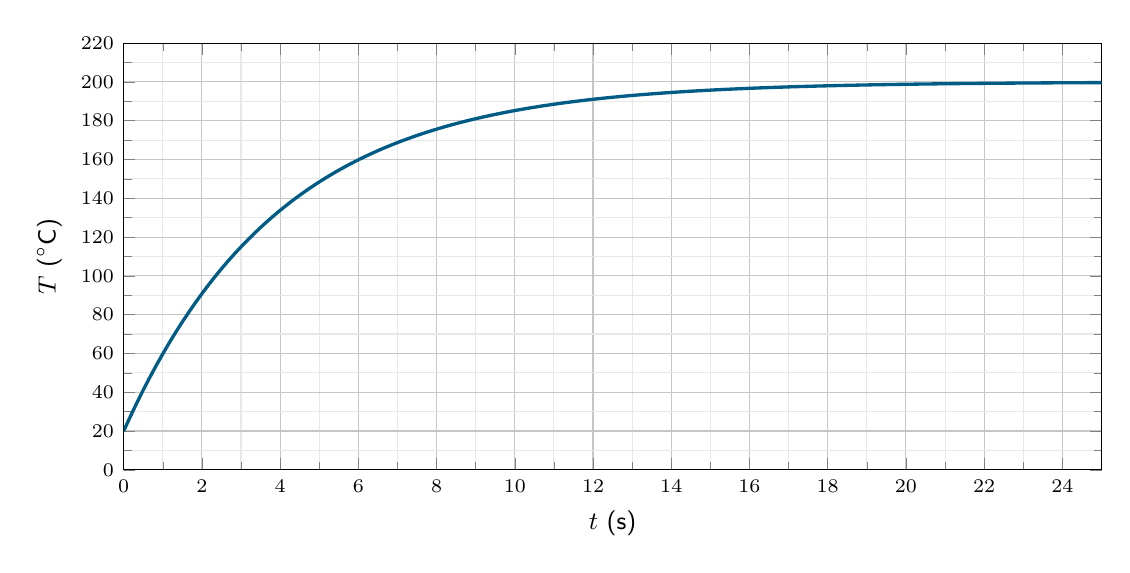
\begin{tikzpicture}
\begin{axis}[width=14cm, height=7cm, xmin=0, xmax=25, ymin=0, ymax=220,
  xtick={0,2,...,24}, ytick={0,20,...,220}, minor x tick num=1, minor y tick num=1,
  grid=both, major grid style={gray!45}, minor grid style={gray!18},
  xlabel={$t$ (s)}, ylabel={$T$ ($^\circ$C)}, tick label style={font=\scriptsize}, label style={font=\small}]
\addplot[uimmblue, very thick, domain=0:25, samples=150] {200-180*exp(-x/4)};
\end{axis}
\end{tikzpicture}
\end{center}
\begin{enumerate}
  \needspace{3.6cm}
  \item Lire la température initiale $T_0$ et la température finale $T_\infty$ indiquée par le capteur.
  \rep{1.5}
  \needspace{4.6cm}
  \item Calculer la température atteinte quand $63\,\%$ de l'évolution est effectuée. En déduire graphiquement la constante de temps $\tau$.
  \rep{2.5}
  \needspace{3.6cm}
  \item Tracer sur le graphique la tangente à la courbe en $t = 0$ (elle passe par $(4\,;\,200)$). Vérifier qu'elle coupe l'asymptote $T = T_\infty$ en $t = \tau$.
  \rep{1.5}
  \needspace{6.6cm}
  \item On admet que $T$ vérifie $\tau\,T' + T = T_\infty$. Écrire cette équation avec les valeurs lues, la résoudre avec la condition initiale, puis contrôler la valeur de $T(4)$ sur la courbe.
  \rep{4}
  \needspace{6.1cm}
  \item Le capteur est considéré comme stabilisé quand l'écart à $T_\infty$ est inférieur à $1\,\%$ de l'évolution totale, soit $1{,}8\,^\circ$C. Calculer ce temps de réponse et le comparer à $5\tau$.
  \rep{3.5}
\end{enumerate}

\exo{Seconds membres non constants}{C5 C6}{[S01] [C01] [C02]}{}
\begin{enumerate}
  \item \textbf{Four en rampe.} La consigne d'un four de revenu monte de $10\,^\circ$C par minute : $\theta_c(t) = 10\,t$. La température $\theta$ de la pièce (en $^\circ$C, $t$ en min) vérifie $\theta' + 0{,}2\,\theta = 2\,t$ et $\theta(0) = 20$.
  \begin{enumerate}
    \needspace{4.6cm}
    \item Chercher une solution particulière de la forme $\theta_p(t) = \beta\,t + \gamma$.
    \rep{3}
    \needspace{4.1cm}
    \item En déduire $\theta(t)$.
    \rep{2.5}
    \needspace{4.6cm}
    \item Pour $t$ grand, comparer $\theta(t)$ à la consigne $10\,t$. De combien de minutes la pièce est-elle en retard sur la consigne ? Comparer ce retard à la constante de temps.
    \rep{2.5}
  \end{enumerate}
  \item \textbf{Produit intermédiaire.} Dans un réacteur, la concentration $y$ d'un produit intermédiaire (en mol/L, $t$ en h) vérifie $y' + 2y = 3\,e^{-t}$ et $y(0) = 0$.
  \begin{enumerate}
    \needspace{5.6cm}
    \item Chercher une solution particulière de la forme $y_p(t) = \lambda\,e^{-t}$, puis résoudre.
    \rep{3.5}
    \needspace{5.6cm}
    \item À quel instant la concentration est-elle maximale ? Quelle est cette valeur maximale ?
    \rep{3.5}
  \end{enumerate}
\end{enumerate}

% ============================================================
\partie{Partie B : applications physiques et industrielles}{Mise en équation, résolution, interprétation. Les exercices 6 à 9 reprennent la version 1 du TD.}
% ============================================================

\exo{Chute d'un composant avec frottement de l'air}{C3 C5 C6}{[S01] [C01] [C02]}{Reprise améliorée de l'exercice 0.1 du TD v1 : mise en équation guidée, critique du modèle.}
\begin{minipage}[t]{0.62\linewidth}
Dans une colonne d'essai, un composant de masse $m = 0{,}5$\,kg est lâché sans vitesse initiale. On étudie son mouvement sur un axe vertical orienté vers le bas (vecteur unitaire $\vec k$). Il subit son poids $\vec P = m\vec g$ et une force de frottement $\vec f = -k\,\vec v$, avec $k = 0{,}1$\,kg/s. On prend $g = 9{,}81\,\text{m/s}^2$.

\medskip
\textbf{Rappel.} Deuxième loi de Newton : $m\,\vec a = \sum \vec F$, où l'accélération est $a(t) = v'(t)$.
\end{minipage}\hfill
\begin{minipage}[t]{0.3\linewidth}\vspace{0pt}\centering
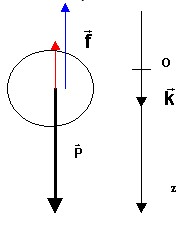
\includegraphics[width=0.75\linewidth]{chute_libre.jpg}
\end{minipage}
\begin{enumerate}
  \needspace{5.1cm}
  \item Projeter la deuxième loi de Newton sur l'axe et montrer que $m\,v'(t) + k\,v(t) = m\,g$.
  \rep{3}
  \needspace{3.6cm}
  \item Écrire l'équation sous forme normalisée. Donner la constante de temps $\tau$.
  \rep{2}
  \needspace{4.6cm}
  \item Résoudre l'équation sachant que $v(0) = 0$.
  \rep{3}
  \needspace{3.6cm}
  \item Déterminer la vitesse limite $v_{\lim}$ lorsque $t \to +\infty$. La convertir en km/h.
  \rep{2}
  \needspace{5.1cm}
  \item Calculer le temps nécessaire pour atteindre $95\,\%$ de la vitesse limite. Comparer à $3\tau$.
  \rep{3}
  \needspace{4.6cm}
  \item Un frottement proportionnel à la vitesse est un bon modèle pour les faibles vitesses. La vitesse limite trouvée vous paraît-elle compatible avec cette hypothèse ? (L'exercice 19 propose un modèle plus réaliste.)
  \rep{2}
\end{enumerate}

\exo{Temporisation par circuit RC dans une armoire de robot}{C1 C3 C5}{[S01] [C01] [C02]}{Reprise améliorée de l'exercice 0.2 du TD v1 : établissement de l'équation, choix d'un composant normalisé.}
\begin{minipage}[t]{0.55\linewidth}
Dans l'armoire de commande d'un robot, un circuit RC série retarde la mise en service d'un module logique. On donne $R = 10\,\text{k}\Omega$, $C = 220\,\mu\text{F}$ et $E = 24$\,V. Le condensateur est déchargé quand on ferme l'interrupteur K à $t = 0$.

\medskip
\textbf{Rappels.} $u_R = R\,i$ ; $i = C\,u_C'$ ; loi des mailles : $E = u_R + u_C$.
\end{minipage}\hfill
\begin{minipage}[t]{0.4\linewidth}\vspace{0pt}\centering
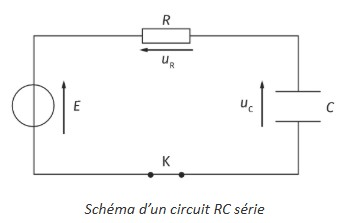
\includegraphics[width=\linewidth]{RC_serie.jpg}
\end{minipage}
\begin{enumerate}
  \needspace{4.1cm}
  \item Montrer que $R\,C\,u_C' + u_C = E$.
  \rep{2.5}
  \needspace{2.8cm}
  \item Calculer la constante de temps $\tau = R\,C$.
  \rep{1.2}
  \needspace{4.6cm}
  \item Résoudre l'équation pour exprimer $u_C(t)$.
  \rep{3}
  \needspace{4.1cm}
  \item Le module logique s'active quand $u_C = 15$\,V. Calculer l'instant d'activation $t_1$.
  \rep{2.5}
  \needspace{4.1cm}
  \item Exprimer l'intensité $i(t) = C\,u_C'(t)$. Calculer $i(0)$.
  \rep{2.5}
  \needspace{6.1cm}
  \item Le cahier des charges impose $t_1 \approx 1$\,s sans changer le condensateur. Calculer la résistance nécessaire, puis choisir la valeur normalisée la plus proche dans la série E12 (\dots ; $3{,}9$ ; $4{,}7$ ; $5{,}6$ ; $6{,}8$\,k$\Omega$ ; \dots). Calculer le $t_1$ obtenu.
  \rep{3.5}
\end{enumerate}

\exo{Refroidissement d'un engrenage après traitement thermique}{C3 C5 C6}{[S01] [C01] [C02] [C03]}{Reprise améliorée de l'exercice 0.3 du TD v1 : identification du coefficient à partir d'une mesure, première simulation Python.}
\begin{minipage}[t]{0.58\linewidth}
Après un traitement par induction, un engrenage en acier sort à $T_0 = 820\,^\circ$C. Il refroidit à l'air dans un atelier à $T_{\text{ext}} = 20\,^\circ$C. On utilise la loi de Newton :
\[
T'(t) = -a\,\big(T(t) - T_{\text{ext}}\big) \qquad (t \text{ en minutes}).
\]
Au pyromètre, on relève $505\,^\circ$C au bout de $10$ minutes.
\end{minipage}\hfill
\begin{minipage}[t]{0.38\linewidth}\vspace{0pt}\centering
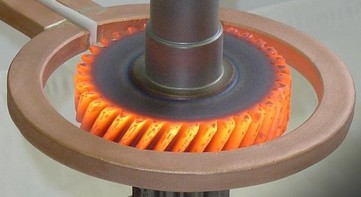
\includegraphics[width=\linewidth]{traitement_thermique.jpg}
\end{minipage}
\begin{enumerate}
  \needspace{4.6cm}
  \item Montrer que $T(t) = 20 + 800\,e^{-a t}$.
  \rep{3}
  \needspace{4.6cm}
  \item À l'aide de la mesure, calculer $a$ (arrondi au millième). Dans la suite, on prend $a = 0{,}05\,\text{min}^{-1}$.
  \rep{2.5}
  \needspace{3.1cm}
  \item Calculer la température de la pièce au bout de $30$ minutes.
  \rep{1.5}
  \needspace{4.6cm}
  \item On ne manipule la pièce sans gants que si $T < 55\,^\circ$C. Combien de temps faut-il attendre ?
  \rep{2.5}
  \needspace{4.6cm}
  \item En été, l'atelier est à $30\,^\circ$C. Reprendre la question 4 et commenter.
  \rep{3}
  \needspace{14cm}
  \item \py{} Le programme ci-dessous calcule $T$ par la méthode d'Euler avec un pas de $5$ minutes, affiche à côté la valeur exacte, puis trace sur un même graphique la solution exacte (courbe) et les valeurs d'Euler (points). Les deux listes \texttt{liste\_t} et \texttt{liste\_T} mémorisent les valeurs calculées à chaque pas ; \texttt{append} ajoute une valeur en fin de liste.
\begin{lstlisting}[style=uimmpython]
import math
import matplotlib.pyplot as plt
a = 0.05        # constante de refroidissement (1/min)
T_ext = 20      # température de l'atelier (°C)
T = 820         # température de la pièce à t = 0 (°C)
t = 0           # temps (min)
dt = 5          # pas de calcul (min)
liste_t = [t]   # instants de calcul
liste_T = [T]   # températures calculées par Euler
while t < 60:
    T = T + dt * (-a * (T - T_ext))     # Euler : T(t+dt) = T(t) + dt * T'(t)
    t = t + dt
    exacte = T_ext + 800 * math.exp(-a * t)            # solution exacte
    print(t, "min :", round(T, 1), "°C   exact :", round(exacte, 1), "°C")
    liste_t.append(t)
    liste_T.append(T)
# Tracé : solution exacte (courbe) et valeurs d'Euler (points)
tt = [k / 10 for k in range(601)]                     # de 0 à 60 min
TT = [T_ext + 800 * math.exp(-a * u) for u in tt]
plt.plot(tt, TT, label="solution exacte")
plt.plot(liste_t, liste_T, "o--", label="Euler, dt = " + str(dt) + " min")
plt.axhline(55, color="red", linestyle=":", label="seuil 55 °C")
plt.xlabel("t (min)")
plt.ylabel("T (°C)")
plt.grid()
plt.legend()
plt.show()
\end{lstlisting}
  \begin{enumerate}
    \item Exécuter le programme. Relever l'écart entre Euler et la valeur exacte à $t = 30$ min.
    \item Sur le graphique, les points d'Euler sont-ils au-dessus ou au-dessous de la courbe exacte ? À quel moment l'écart semble-t-il le plus grand ? À l'aide de la forme de la courbe, expliquer pourquoi Euler se trompe toujours dans le même sens.
    \item Remplacer \texttt{dt = 5} par \texttt{dt = 1} et relancer. Que constate-t-on sur les valeurs et sur le graphique ?
  \end{enumerate}
  \rep{4}
  \needspace{3.2cm}
  \item À $820\,^\circ$C, la pièce est rouge : elle perd aussi beaucoup de chaleur par rayonnement, phénomène que la loi de Newton ne prend pas en compte. Le modèle sous-estime-t-il ou surestime-t-il la vitesse de refroidissement au début ? (L'exercice 20 reprend cette question.)
  \rep{2}
\end{enumerate}

\exo{Moteur de l'axe J1 d'un robot FANUC}{C3 C5 C6}{[S01] [C01] [C02]}{Reprise améliorée de l'exercice 0.4 du TD v1 : tracé guidé, confrontation à un cahier des charges.}
\begin{minipage}[t]{0.5\linewidth}
L'axe J1 fait tourner la base du robot. Dans un modèle simplifié, la vitesse angulaire $\omega(t)$ (en rad/s) de son moteur à courant continu vérifie :
\[
J\,\omega' + f\,\omega = K\,u .
\]
Données : inertie $J = 0{,}02\,\text{kg}\cdot\text{m}^2$ ; frottement $f = 0{,}01\,\text{N}\cdot\text{m}\cdot\text{s/rad}$ ; constante $K = 0{,}5\,\text{N}\cdot\text{m/V}$ ; tension de commande $u = 12$\,V (échelon). Le moteur est à l'arrêt à $t = 0$.
\end{minipage}\hfill
\begin{minipage}[t]{0.45\linewidth}\vspace{0pt}\centering
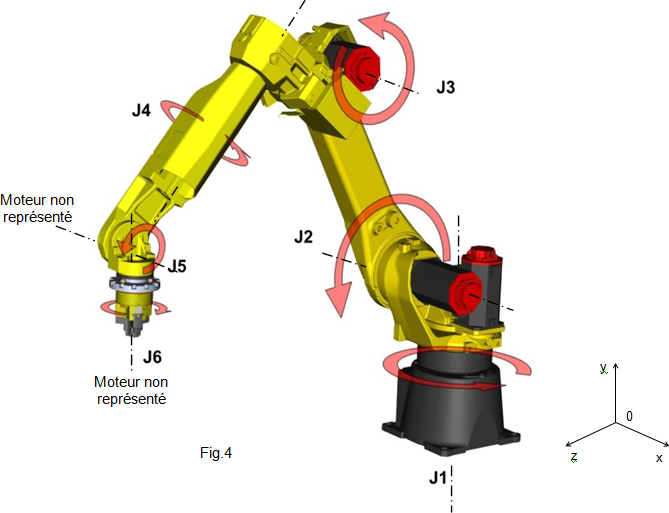
\includegraphics[width=\linewidth]{Robot_FANUC_M20iA-4.png}
\end{minipage}
\begin{enumerate}
  \needspace{5.1cm}
  \item Mettre l'équation sous la forme canonique $\tau\,\omega' + \omega = \Omega_0$. Calculer $\tau$ et $\Omega_0$.
  \rep{3}
  \needspace{3.6cm}
  \item Donner la solution $\omega(t)$.
  \rep{2}
  \item Calculer la pente de la tangente à l'origine, puis tracer sur le repère ci-dessous l'asymptote, la tangente à l'origine et la courbe $\omega(t)$.
\end{enumerate}
\begin{center}
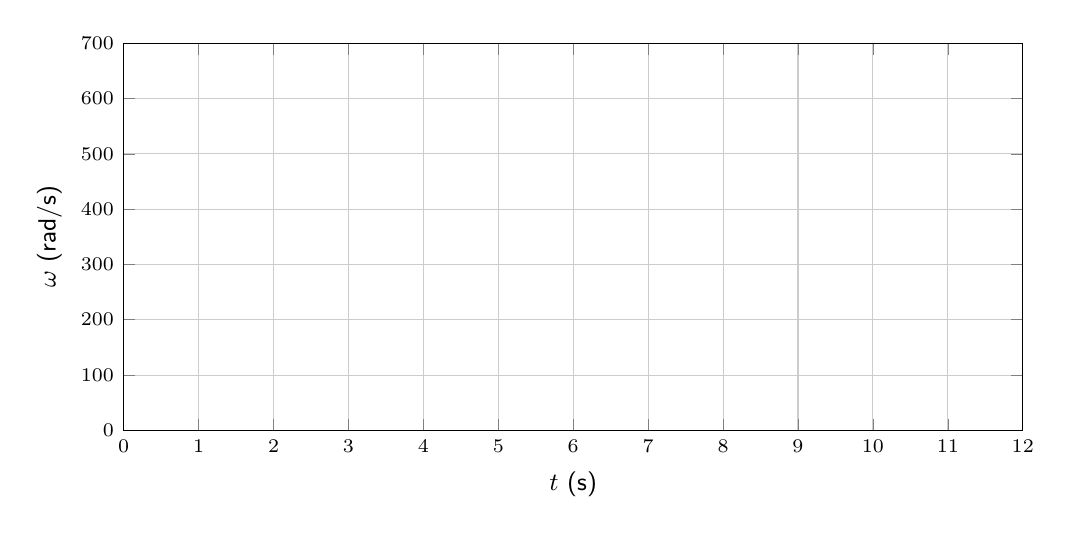
\begin{tikzpicture}
\begin{axis}[width=13cm, height=6.5cm, xmin=0, xmax=12, ymin=0, ymax=700,
  xtick={0,1,...,12}, ytick={0,100,...,700}, grid=both, major grid style={gray!40},
  xlabel={$t$ (s)}, ylabel={$\omega$ (rad/s)}, tick label style={font=\scriptsize}, label style={font=\small}]
\addplot[draw=none] coordinates {(0,0)};
\end{axis}
\end{tikzpicture}
\end{center}
\begin{enumerate}[resume]
  \needspace{3.6cm}
  \item Calculer le temps de réponse à $5\,\%$.
  \rep{2}
  \needspace{6.6cm}
  \item Le cahier des charges exige un temps de réponse à $5\,\%$ inférieur ou égal à $0{,}6$\,s. Le moteur seul convient-il ? Un correcteur électronique revient à multiplier $f$ et $K$ par $10$. Calculer la nouvelle constante de temps et la nouvelle vitesse finale. Le cahier des charges est-il respecté ?
  \rep{3.5}
\end{enumerate}

\exo{Ouverture et fermeture d'une électrovanne}{C3 C5 C6}{[S01] [C01] [C02]}{}
\begin{minipage}[t]{0.56\linewidth}
La bobine d'une électrovanne pneumatique est modélisée par une inductance $L = 0{,}5$\,H en série avec une résistance $R = 25\,\Omega$. Elle est alimentée sous $E = 24$\,V à $t = 0$, avec $i(0) = 0$. La vanne s'ouvre quand l'intensité atteint $0{,}6$\,A.

\medskip
\textbf{Rappel.} La tension aux bornes d'une inductance vaut $u_L = L\,i'$.
\end{minipage}\hfill
\begin{minipage}[t]{0.4\linewidth}\vspace{0pt}\centering
\begin{circuitikz}[scale=0.8, transform shape]
\draw (0,0) to[V, l=$E$] (0,3) to[R, l=$R$] (3,3) to[L, l=$L$] (3,0) -- (0,0);
\draw[-{Latex}] (0.6,3.35) -- node[above]{$i$} (1.2,3.35);
\end{circuitikz}
\end{minipage}
\begin{enumerate}
  \needspace{3.6cm}
  \item À l'aide de la loi des mailles, montrer que $L\,i' + R\,i = E$.
  \rep{2}
  \needspace{3.6cm}
  \item Calculer la constante de temps $\tau$ et l'intensité $I_\infty$ du régime permanent.
  \rep{2}
  \needspace{5.1cm}
  \item Exprimer $i(t)$. Calculer le temps d'ouverture de la vanne (en ms).
  \rep{3.5}
  \needspace{6.6cm}
  \item On coupe l'alimentation quand le régime permanent est atteint. On prend cet instant comme nouvelle origine des temps. Le courant s'éteint alors à travers une diode de roue libre et vérifie $L\,i' + R\,i = 0$, avec $i(0) = I_\infty$. La vanne se referme quand $i < 0{,}2$\,A. Calculer le temps de fermeture.
  \rep{3.5}
  \needspace{4.1cm}
  \item Sans diode, le courant serait coupé presque instantanément. En utilisant $u_L = L\,i'$, expliquer le risque pour le transistor de commande.
  \rep{2}
\end{enumerate}

\exo{Filtrer le signal d'un capteur}{C5 C6}{[S01] [C01]}{}
Le signal d'un capteur est perturbé par des parasites. On le fait passer dans un filtre RC de constante de temps $\tau = 10^{-3}$\,s. La tension de sortie $u$ (en V) vérifie
\[
\tau\,u' + u = e(t), \qquad e(t) = 5\sin(\omega t), \qquad \omega = 1\,000\ \text{rad/s}, \qquad u(0) = 0 .
\]
\begin{enumerate}
  \needspace{3.1cm}
  \item Vérifier que $\omega\tau = 1$ et écrire l'équation avec les valeurs numériques.
  \rep{1.5}
  \needspace{7.1cm}
  \item On cherche une solution particulière $u_p(t) = \lambda\cos(1000\,t) + \mu\sin(1000\,t)$. En identifiant les coefficients de $\cos$ et de $\sin$, montrer que $\lambda = -2{,}5$ et $\mu = 2{,}5$.
  \rep{4.5}
  \needspace{5.1cm}
  \item En déduire $u(t)$ avec la condition initiale. Après combien de temps le terme transitoire est-il négligeable ($5\tau$) ?
  \rep{3}
  \needspace{4.6cm}
  \item On admet que $a\sin x - a\cos x = a\sqrt{2}\,\sin\!\left(x - \frac{\pi}{4}\right)$. Écrire $u_p$ sous cette forme. Donner l'amplitude du signal filtré et la comparer à celle de $e$.
  \rep{2.5}
  \needspace{6.6cm}
  \item On admet que, pour une pulsation $\omega$ quelconque, l'amplitude du régime permanent vaut
  \[ A(\omega) = \frac{5}{\sqrt{1 + (\omega\tau)^2}} . \]
  Calculer cette amplitude pour un parasite de pulsation $10\,000$\,rad/s. Quel est le rôle du filtre ?
  \rep{3}
\end{enumerate}

% ============================================================
\partie{Partie C : au-delà du cours}{Équations du premier ordre non linéaires ou à coefficient variable. Chaque étape est guidée ; quand le calcul exact devient impossible, la méthode d'Euler prend le relais.}

\begin{tcolorbox}[colback=uimmlightgray, colframe=uimmgray, boxrule=0.6pt, arc=2pt, left=8pt, right=8pt, top=4pt, bottom=4pt, title={\bfseries Méthodes pour les équations non linéaires du premier ordre}, coltitle=white, colbacktitle=uimmgray]
\small
\textbf{Variables séparables} : l'équation s'écrit $g(y)\,y' = f(x)$. On écrit $y' = \dfrac{\dd y}{\dd x}$, on sépare $g(y)\,\dd y = f(x)\,\dd x$, on intègre chaque membre, puis on isole $y$. Astuce : écrire la constante sous la forme $\ln|K|$ quand des logarithmes apparaissent.

\smallskip
\textbf{Équation homogène} : l'équation s'écrit $y' = f\!\left(\dfrac{y}{x}\right)$. On pose $t = \dfrac{y}{x}$, soit $y = t\,x$ et $y' = t + x\,t'$. On obtient $x\,t' = f(t) - t$, qui est à variables séparables.

\smallskip
\textbf{Équation de Bernoulli} : l'équation s'écrit $y' + a(x)\,y = b(x)\,y^{\alpha}$ avec $\alpha \neq 0$ et $\alpha \neq 1$. On divise par $y^{\alpha}$ et on pose $z = y^{1-\alpha}$, d'où $z' = (1-\alpha)\,y^{-\alpha}\,y'$. L'équation en $z$ est linéaire.

\smallskip
\textbf{Méthode d'Euler} : si aucune primitive n'est accessible, ou si $y$ ne peut pas être isolé, on calcule une solution approchée pas à pas.
\end{tcolorbox}

\exo{Variables séparables : la méthode}{C4 C5}{[S01] [C01] [C02]}{}
On applique la méthode des variables séparables (encadré ci-dessus) à trois équations. La variable est $x$.
\begin{enumerate}
  \needspace{5cm}
  \item On considère $x\,y' = 3\,y$ sur $]0\,;\,+\infty[$, avec $y(1) = 2$.
  \begin{enumerate}
    \item Pour $y \neq 0$, montrer que l'équation s'écrit $\dfrac{\dd y}{y} = 3\,\dfrac{\dd x}{x}$.
    \rep{2}
    \item Intégrer chaque membre. En écrivant la constante sous la forme $\ln|K|$, montrer que $y = K\,x^3$. Vérifier que la fonction nulle est aussi solution.
    \rep{3}
    \item Déterminer la solution vérifiant $y(1) = 2$.
    \rep{1.5}
  \end{enumerate}
  \needspace{4cm}
  \item On considère $y\,y' = x$ avec $y(0) = 2$. Séparer les variables, intégrer, puis montrer que $y(x) = \sqrt{x^2 + 4}$.
  \rep{3.5}
  \needspace{5cm}
  \item On considère $y' = 2x\,y^2$ avec $y(0) = 1$.
  \begin{enumerate}
    \item Séparer les variables. Vérifier qu'une primitive de $y \mapsto \dfrac{1}{y^2}$ est $y \mapsto -\dfrac{1}{y}$.
    \rep{2.5}
    \item En déduire que $y(x) = \dfrac{1}{1 - x^2}$.
    \rep{2.5}
    \item Sur quel intervalle contenant $0$ cette solution est-elle définie ? Que se passe-t-il quand $x$ tend vers $1$ ? Les solutions des équations linéaires du cours présentent-elles ce comportement ?
    \rep{2.5}
  \end{enumerate}
\end{enumerate}

\exo{Usure d'un bain de traitement de surface (cinétique d'ordre 2)}{C3 C5 C6}{[S01] [C01] [C02]}{}
Dans un bain de traitement de surface, un additif se décompose au cours du temps. On admet que sa concentration $c(t)$ (en mol/L, $t$ en min) suit une cinétique d'ordre 2 :
\[
c'(t) = -k\,c(t)^2, \qquad k = 0{,}05\ \text{L}\cdot\text{mol}^{-1}\cdot\text{min}^{-1}, \qquad c(0) = c_0 = 2\ \text{mol/L}.
\]
\begin{enumerate}
  \needspace{3.5cm}
  \item Pourquoi cette équation n'est-elle pas linéaire ? Montrer qu'elle est à variables séparables.
  \rep{2}
  \needspace{5cm}
  \item Résoudre l'équation : montrer que $\dfrac{1}{c(t)} = \dfrac{1}{c_0} + k\,t$, puis que $c(t) = \dfrac{c_0}{1 + k\,c_0\,t}$.
  \rep{3.5}
  \needspace{3.5cm}
  \item Calculer le temps de demi-réaction $t_{1/2}$, instant où la concentration a diminué de moitié.
  \rep{2}
  \needspace{3.5cm}
  \item Le bain doit être régénéré quand $c < 0{,}1$\,mol/L. Au bout de combien de temps ?
  \rep{2}
  \needspace{4.5cm}
  \item Montrer que $t_{1/2} = \dfrac{1}{k\,c_0}$. Que devient $t_{1/2}$ si $c_0 = 4$\,mol/L ? Pour une cinétique d'ordre 1 ($c' = -k\,c$), $t_{1/2} = \dfrac{\ln 2}{k}$ ne dépend pas de $c_0$. En utilisant la question 2, proposer un tracé qui permet de reconnaître expérimentalement une cinétique d'ordre 2.
  \rep{3.5}
\end{enumerate}

\exo{Vidange d'un réservoir de lubrifiant (loi de Torricelli)}{C2 C3 C4 C5 C6}{[S01] [C01] [C02]}{Reprise améliorée de l'exercice 0.5 du TD v1 : le modèle linéaire est remplacé par la loi physique d'écoulement.}
\begin{minipage}[t]{0.64\linewidth}
La version 1 du TD utilisait le modèle $h' + 0{,}2\,h = 0$. Avec ce modèle, le réservoir ne se vide jamais complètement.

Pour un écoulement libre par un orifice au fond, la vitesse de sortie du liquide vaut $\sqrt{2 g h}$ (loi de Torricelli). Le débit est donc proportionnel à $\sqrt{h}$ et la hauteur $h$ (en m, $t$ en min) vérifie :
\[
h'(t) = -k\sqrt{h(t)}, \qquad k = 0{,}1\ \text{m}^{1/2}\cdot\text{min}^{-1}, \qquad h(0) = 1{,}5 .
\]
\end{minipage}\hfill
\begin{minipage}[t]{0.32\linewidth}\vspace{0pt}\centering
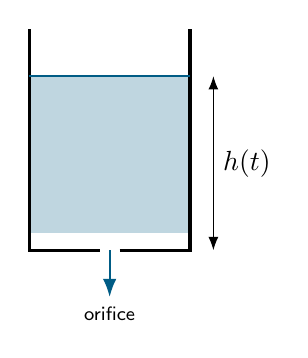
\begin{tikzpicture}[scale=0.85]
\fill[uimmblue!25] (0,0.25) rectangle (2.4,2.6);
\draw[very thick] (0,3.3) -- (0,0) -- (1.05,0); \draw[very thick] (1.35,0) -- (2.4,0) -- (2.4,3.3);
\draw[uimmblue, thick] (0,2.6) -- (2.4,2.6);
\draw[{Latex}-{Latex}] (2.75,0) -- node[right]{$h(t)$} (2.75,2.6);
\draw[uimmblue, thick, -{Latex}] (1.2,0) -- (1.2,-0.7);
\node[below, font=\scriptsize] at (1.2,-0.7) {orifice};
\end{tikzpicture}
\end{minipage}
\begin{enumerate}
  \needspace{4.1cm}
  \item Pourquoi cette équation n'est-elle pas linéaire ? Peut-on appliquer directement les méthodes du cours ?
  \rep{2}
  \item \textbf{Changement de variable.} On pose $u(t) = \sqrt{h(t)}$.
  \begin{enumerate}
    \needspace{4.6cm}
    \item On rappelle que la dérivée de $\sqrt{h(t)}$ est $\dfrac{h'(t)}{2\sqrt{h(t)}}$. Montrer que $u'(t) = -\dfrac{k}{2}$.
    \rep{2.5}
    \needspace{5.1cm}
    \item En déduire $u(t)$ avec $u(0) = \sqrt{1{,}5}$, puis montrer que $h(t) = \left(\sqrt{1{,}5} - 0{,}05\,t\right)^2$.
    \rep{3}
  \end{enumerate}
  \needspace{4.6cm}
  \item Vérifier par le calcul de $h'(t)$ que cette fonction est bien solution, tant que $\sqrt{1{,}5} - 0{,}05\,t \geq 0$.
  \rep{2.5}
  \needspace{3.6cm}
  \item Calculer la durée $T_v$ de la vidange complète.
  \rep{2}
  \needspace{5.6cm}
  \item Calculer le temps nécessaire pour que le niveau baisse de moitié, puis l'instant où l'alarme «~niveau critique~» ($h < 0{,}1$\,m) se déclenche.
  \rep{3.5}
  \needspace{8.2cm}
  \item \py{} Exécuter le programme suivant, qui résout l'équation par la méthode d'Euler. Comparer avec la question 5.
\begin{lstlisting}[style=uimmpython]
import math
k = 0.1         # coefficient de vidange (m^0,5 par minute)
h = 1.5         # hauteur initiale (m)
t = 0           # temps (min)
dt = 0.01       # pas de calcul (min)
while h > 0.1:
    h = h - dt * k * math.sqrt(h)      # Euler : h(t+dt) = h(t) + dt * h'(t)
    t = t + dt
print("Alarme déclenchée à t =", round(t, 2), "min")
\end{lstlisting}
  \rep{1.5}
  \needspace{5.6cm}
  \item Avec le modèle linéaire de la version 1 ($h' + 0{,}2\,h = 0$), on trouvait $3{,}47$\,min pour la mi-hauteur et $13{,}54$\,min pour l'alarme. Comparer les deux modèles. Lequel décrit le mieux un réservoir qui se vide par gravité ? Justifier.
  \rep{3}
\end{enumerate}

\exo{Dépollution d'une cuve à volume variable (coefficient variable)}{C1 C3 C4 C5 C6}{[S01] [C01] [C02]}{Reprise améliorée de l'exercice 0.6 du TD v1 : méthode de séparation des variables détaillée, seuil de rejet, simulation.}
\begin{minipage}[t]{0.6\linewidth}
Une cuve de traitement des eaux contient initialement $V_0 = 1\,000$\,L d'eau polluée par $m_0 = 5$\,kg de solvant. On injecte de l'eau pure avec un débit $Q_e = 20$\,L/min. Une pompe aspire le mélange, supposé homogène, avec un débit $Q_s = 25$\,L/min. On note $m(t)$ la masse de solvant (en kg) dans la cuve à l'instant $t$ (en min).
\end{minipage}\hfill
\begin{minipage}[t]{0.36\linewidth}\vspace{0pt}\centering
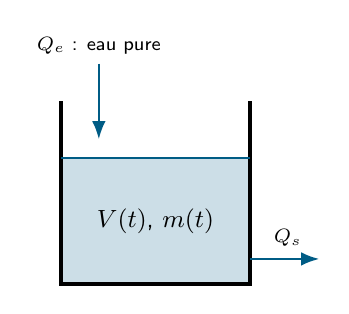
\begin{tikzpicture}[scale=0.8]
\fill[uimmblue!20] (0,0) rectangle (3,2);
\draw[very thick] (0,2.9) -- (0,0) -- (3,0) -- (3,2.9);
\draw[uimmblue, thick] (0,2) -- (3,2);
\draw[uimmblue, thick, -{Latex}] (0.6,3.5) -- (0.6,2.3);
\node[above, font=\scriptsize] at (0.6,3.5) {$Q_e$ : eau pure};
\draw[uimmblue, thick, -{Latex}] (3,0.4) -- (4.1,0.4);
\node[above, font=\scriptsize] at (3.6,0.45) {$Q_s$};
\node[font=\small] at (1.5,1) {$V(t)$, $m(t)$};
\end{tikzpicture}
\end{minipage}
\begin{enumerate}
  \needspace{4.6cm}
  \item \textbf{Volume.} Sachant que $V'(t) = Q_e - Q_s$, exprimer $V(t)$. À quel instant la cuve est-elle vide ? On travaille dans la suite sur $[0\,;\,200[$.
  \rep{2.5}
  \needspace{5.6cm}
  \item \textbf{Mise en équation.} On admet que $m'(t) = -Q_s\,\dfrac{m(t)}{V(t)}$. Montrer que $m'(t) + \dfrac{5}{200 - t}\,m(t) = 0$. Pourquoi les méthodes du cours ne s'appliquent-elles pas directement ?
  \rep{3}
  \item \textbf{Résolution guidée.} L'équation est à variables séparables (méthode de l'exercice 12). On suppose $m(t) > 0$.
  \begin{enumerate}
    \needspace{4.6cm}
    \item Justifier que la dérivée de $\ln\big(m(t)\big)$ est $\dfrac{m'(t)}{m(t)}$, puis que $\dfrac{m'(t)}{m(t)} = -\dfrac{5}{200 - t}$.
    \rep{2.5}
    \needspace{4.1cm}
    \item Vérifier que $t \mapsto 5\ln(200 - t)$ est une primitive de $t \mapsto -\dfrac{5}{200 - t}$ sur $[0\,;\,200[$.
    \rep{2}
    \needspace{4.6cm}
    \item En déduire qu'il existe une constante $c$ telle que $\ln\big(m(t)\big) = 5\ln(200 - t) + c$, puis que $m(t) = A\,(200 - t)^5$ avec $A > 0$.
    \rep{2.5}
    \needspace{3.6cm}
    \item Avec $m(0) = 5$, montrer que $m(t) = 5\left(\dfrac{200 - t}{200}\right)^5$.
    \rep{2}
  \end{enumerate}
  \needspace{5.6cm}
  \item \textbf{Concentration.} On note $c(t) = \dfrac{m(t)}{V(t)}$ la concentration en solvant. Montrer qu'en g/L :
  \[ c(t) = 5\left(\frac{200 - t}{200}\right)^4 . \]
  \rep{3}
  \needspace{5.1cm}
  \item On suppose que le rejet du mélange est autorisé quand $c \leq 0{,}5$\,g/L. Calculer l'instant $t_s$ où ce seuil est atteint et le volume restant dans la cuve.
  \rep{3}
  \needspace{7.7cm}
  \item \py{} Exécuter le programme suivant et comparer avec la question 5.
\begin{lstlisting}[style=uimmpython]
m = 5           # masse de solvant (kg)
V = 1000        # volume dans la cuve (L)
t = 0           # temps (min)
dt = 0.01       # pas de calcul (min)
while m / V > 0.0005:                  # tant que la concentration dépasse 0,5 g/L
    m = m - dt * 25 * m / V            # Euler : m'(t) = -Qs * m / V
    V = V - dt * 5                     # V'(t) = Qe - Qs = -5 L/min
    t = t + dt
print("c < 0,5 g/L après", round(t, 1), "min ; volume restant :", round(V), "L")
\end{lstlisting}
  \rep{1.5}
  \needspace{6.6cm}
  \item \textbf{Autre réglage.} Si l'on règle $Q_s = 20$\,L/min, le volume reste constant et $m' = -0{,}02\,m$. Calculer l'instant où la concentration passe sous $0{,}5$\,g/L. Comparer les deux réglages (durée, volume à traiter ensuite).
  \rep{4}
  \needspace{4.1cm}
  \item Que vaut la masse de solvant restante quand la cuve se vide ($t \to 200$) ? Ce résultat est-il physiquement cohérent ?
  \rep{2}
\end{enumerate}

\exo{Une équation homogène : $y' = \left(\frac{y}{x}\right)^2$}{C3 C4 C5}{[S01] [C01] [C02] [C03]}{}
On cherche les fonctions $y$ définies pour $x > 0$ telles que $x^2\,y' = y^2$ et $y(1) = \dfrac12$.
\begin{enumerate}
  \needspace{3cm}
  \item Montrer que l'équation s'écrit $y' = \left(\dfrac{y}{x}\right)^2$. Est-elle linéaire ? Vérifier que $y'$ ne dépend de $x$ et de $y$ que par le quotient $\dfrac{y}{x}$ : l'équation est homogène.
  \rep{2}
  \needspace{5cm}
  \item \textbf{Changement de fonction.} On pose $t(x) = \dfrac{y(x)}{x}$, donc $y = t\,x$.
  \begin{enumerate}
    \item Montrer que $y' = t + x\,t'$.
    \rep{1.5}
    \item En déduire que $t$ vérifie $x\,t' = t^2 - t$. Cette équation est-elle à variables séparables ?
    \rep{2}
  \end{enumerate}
  \needspace{4cm}
  \item \textbf{Résolution en $t$.}
  \begin{enumerate}
    \item Vérifier que les fonctions constantes $t = 0$ et $t = 1$ sont solutions. Quelles fonctions $y$ leur correspondent ? Les vérifier dans l'équation de départ.
    \rep{2.5}
    \item Pour $t \neq 0$ et $t \neq 1$, séparer les variables : $\dfrac{\dd t}{t^2 - t} = \dfrac{\dd x}{x}$. Vérifier que $\dfrac{1}{t^2 - t} = \dfrac{1}{t - 1} - \dfrac{1}{t}$.
    \rep{2.5}
    \item Intégrer et montrer que $\dfrac{t - 1}{t} = K\,x$ ($K$ constante réelle).
    \rep{2.5}
    \item En déduire $t = \dfrac{1}{1 - K x}$, puis $y = \dfrac{x}{1 - K x}$.
    \rep{2}
  \end{enumerate}
  \needspace{3.5cm}
  \item Déterminer la solution vérifiant $y(1) = \frac12$. Vérifier par le calcul qu'elle satisfait $x^2\,y' = y^2$.
  \rep{3}
  \needspace{9cm}
  \item \py{} Le programme suivant trace quelques courbes de la famille $y = \dfrac{x}{1 - Kx}$ pour $K \leq 0$. Exécuter le programme. Vers quelle valeur chaque courbe tend-elle quand $x$ devient grand ? Le démontrer pour $K < 0$.
\begin{lstlisting}[style=uimmpython]
import matplotlib.pyplot as plt
xs = [j / 100 for j in range(1, 501)]          # x de 0,01 à 5
for K in [-2, -1, -0.5, 0]:
    ys = [x / (1 - K * x) for x in xs]
    plt.plot(xs, ys, label="K = " + str(K))
plt.xlabel("x")
plt.ylabel("y")
plt.legend()
plt.show()
\end{lstlisting}
  \rep{2.5}
  \needspace{4cm}
  \item \textbf{Contrôle par une autre méthode.} Cette équation particulière est aussi à variables séparables : $\dfrac{y'}{y^2} = \dfrac{1}{x^2}$. La résoudre directement et comparer avec la question 3. Pourquoi la méthode du changement $y = t\,x$ reste-t-elle utile en général ?
  \rep{3.5}
\end{enumerate}

\exo{Contamination d'un fluide de coupe (modèle logistique)}{C3 C4 C5}{[S01] [C01] [C02] [C03]}{}
L'émulsion d'huile soluble d'un centre d'usinage se contamine par des bactéries. On note $N(t)$ leur concentration (en UFC/mL, unités formant colonie) au jour $t$. On utilise le modèle logistique de Verhulst :
\[
N'(t) = r\,N(t)\left(1 - \frac{N(t)}{K}\right), \qquad r = 0{,}8\ \text{jour}^{-1}, \qquad K = 10^8\ \text{UFC/mL}, \qquad N(0) = 10^3 .
\]
On suppose que le service maintenance déclenche un traitement de l'émulsion quand $N$ dépasse $10^6$\,UFC/mL.
\begin{enumerate}
  \needspace{5.6cm}
  \item \textbf{Phase de démarrage.} Tant que $N$ est très petit devant $K$, on a $1 - \frac{N}{K} \approx 1$. Écrire l'équation approchée, la résoudre et estimer la date du traitement.
  \rep{3.5}
  \needspace{4.1cm}
  \item Vérifier que les fonctions constantes $N = 0$ et $N = K$ sont solutions. Interpréter $K$.
  \rep{2}
  \item \textbf{Changement de variable.} L'équation s'écrit $N' - r\,N = -\frac{r}{K}\,N^2$ : c'est une équation de Bernoulli avec $\alpha = 2$. On pose donc $z = N^{1-\alpha} = \dfrac{1}{N(t)}$.
  \begin{enumerate}
    \needspace{5.1cm}
    \item Montrer que $z' = -\dfrac{N'}{N^2}$, puis que $z' + r\,z = \dfrac{r}{K}$.
    \rep{3.5}
    \needspace{4.1cm}
    \item Résoudre cette équation linéaire avec $z(0) = 10^{-3}$.
    \rep{2.5}
    \needspace{4.6cm}
    \item En déduire que $N(t) = \dfrac{K}{1 + \left(\frac{K}{N_0} - 1\right)e^{-r t}}$ avec $N_0 = 10^3$.
    \rep{2.5}
  \end{enumerate}
  \needspace{5.1cm}
  \item Calculer la date exacte du traitement. Comparer avec la question 1 et expliquer pourquoi les deux résultats sont proches.
  \rep{3}
  \needspace{4.6cm}
  \item Calculer l'instant où $N = \frac{K}{2}$ (c'est le moment où la contamination progresse le plus vite).
  \rep{2.5}
  \needspace{7.5cm}
  \item \py{} Exécuter les deux programmes suivants.
\begin{lstlisting}[style=uimmpython]
r = 0.8         # taux de croissance (par jour)
K = 1e8         # capacité maximale du fluide (UFC/mL)
N = 1e3         # contamination initiale (UFC/mL)
t = 0           # temps (jours)
dt = 0.01       # pas de calcul (jour)
while N < 1e6:
    N = N + dt * r * N * (1 - N / K)   # Euler : N(t+dt) = N(t) + dt * N'(t)
    t = t + dt
print("Seuil de 1 000 000 UFC/mL atteint après", round(t, 2), "jours")
\end{lstlisting}
\needspace{6.5cm}
\begin{lstlisting}[style=uimmpython]
import math
import matplotlib.pyplot as plt
r = 0.8
K = 1e8
temps = [j / 10 for j in range(301)]            # de 0 à 30 jours
for N0 in [1e2, 1e3, 1e4, 1e5]:
    N = [K / (1 + (K / N0 - 1) * math.exp(-r * t)) for t in temps]
    plt.plot(temps, N, label="N0 = " + str(int(N0)))
plt.xlabel("t (jours)")
plt.ylabel("N (UFC/mL)")
plt.legend()
plt.show()
\end{lstlisting}
  \begin{enumerate}
    \item Comparer le résultat du premier programme avec la question 4.
    \item Le second trace la famille des courbes solutions pour quatre contaminations initiales. Décrire leur point commun et ce qui les distingue. Quel intérêt y a-t-il à changer l'émulsion avec un circuit bien nettoyé ?
  \end{enumerate}
  \rep{3.5}
\end{enumerate}

\exo{Ralentissement d'un volant d'inertie (équation de Bernoulli)}{C3 C4 C5 C6}{[S01] [C01] [C02]}{}
Après coupure du moteur, le volant d'inertie d'une presse ralentit sous l'effet de deux couples résistants : un frottement visqueux $f\,\omega$ et un couple aérodynamique $c\,\omega^2$. Sa vitesse angulaire $\omega(t)$ (en rad/s, $t$ en s) vérifie :
\[
J\,\omega' = -f\,\omega - c\,\omega^2, \qquad J = 0{,}5\ \text{kg}\cdot\text{m}^2, \quad f = 0{,}05\ \text{N}\cdot\text{m}\cdot\text{s}, \quad c = 0{,}001\ \text{N}\cdot\text{m}\cdot\text{s}^2, \quad \omega(0) = 300 .
\]
\begin{enumerate}
  \needspace{3.5cm}
  \item Montrer que $\omega' + 0{,}1\,\omega = -0{,}002\,\omega^2$. Identifier $a$, $b$ et $\alpha$ dans la forme de Bernoulli $y' + a\,y = b\,y^{\alpha}$.
  \rep{2}
  \needspace{5cm}
  \item \textbf{Changement de fonction.} On pose $z = \omega^{1-\alpha} = \dfrac{1}{\omega}$.
  \begin{enumerate}
    \item Montrer que $z' = -\dfrac{\omega'}{\omega^2}$.
    \rep{1.5}
    \item Diviser l'équation par $\omega^2$ et en déduire que $z' - 0{,}1\,z = 0{,}002$.
    \rep{2.5}
  \end{enumerate}
  \needspace{5cm}
  \item Résoudre cette équation linéaire avec $z(0) = \dfrac{1}{300}$. En déduire que $\omega(t) = \dfrac{300}{7\,e^{0{,}1 t} - 6}$.
  \rep{4}
  \needspace{3cm}
  \item Calculer le temps nécessaire pour que la vitesse descende à $30$\,rad/s.
  \rep{2}
  \needspace{4cm}
  \item Sans couple aérodynamique ($c = 0$), on aurait $\omega(t) = 300\,e^{-0{,}1 t}$. Calculer le même temps. Comparer les deux couples résistants à $300$\,rad/s et expliquer l'écart.
  \rep{3}
  \needspace{3.5cm}
  \item Montrer que, pour $t$ grand, $\omega(t) \approx \dfrac{300}{7}\,e^{-0{,}1 t}$. Interpréter : quel couple résistant domine en fin de ralentissement ?
  \rep{3}
\end{enumerate}

\exo{Essai de chute d'un boîtier : frottement quadratique}{C2 C3 C4 C5}{[S01] [C01]}{}
À grande vitesse, la force de frottement de l'air est proportionnelle au \textbf{carré} de la vitesse. On réalise un essai de chute d'un boîtier électronique de masse $m = 2$\,kg, largué sans vitesse initiale depuis un drone. Sur un axe vertical orienté vers le bas, le boîtier subit son poids et une force de frottement de valeur $k\,v^2$, opposée au mouvement, avec $k = 0{,}02$\,kg/m. On prend $g = 9{,}81\,\text{m/s}^2$.
\begin{enumerate}
  \needspace{4.6cm}
  \item Montrer avec la deuxième loi de Newton que $v'(t) = g - \dfrac{k}{m}\,v(t)^2$. Pourquoi cette équation n'est-elle pas linéaire ?
  \rep{2.5}
  \needspace{4.1cm}
  \item Au tout début de la chute, $v$ est proche de $0$. Que vaut alors $v'$ ? Quel mouvement retrouve-t-on ?
  \rep{2}
  \needspace{4.6cm}
  \item En régime permanent, la vitesse est constante, donc $v' = 0$. En déduire la vitesse limite $v_{\lim} = \sqrt{\dfrac{m\,g}{k}}$. Calculer sa valeur en m/s et en km/h.
  \rep{2.5}
  \needspace{10.5cm}
  \item \py{} Cette équation est à variables séparables, mais la primitive de $\dfrac{1}{g - \frac{k}{m}v^2}$ demande un calcul long. On la résout d'abord numériquement. Exécuter le programme suivant et relever l'instant où le boîtier atteint $95\,\%$ de $v_{\lim}$, ainsi que la hauteur de chute nécessaire.
\begin{lstlisting}[style=uimmpython]
g = 9.81        # pesanteur (m/s²)
m = 2.0         # masse du boîtier (kg)
k = 0.02        # coefficient de traînée (kg/m)
v, z, t = 0, 0, 0     # vitesse, distance, temps au départ
dt = 0.001      # pas de calcul (s)
v_lim = (m * g / k) ** 0.5
while v < 0.95 * v_lim:
    a = g - (k / m) * v ** 2       # accélération v'(t)
    v = v + a * dt                 # Euler sur la vitesse
    z = z + v * dt                 # Euler sur la distance
    t = t + dt
print("v_lim =", round(v_lim, 2), "m/s")
print("95 % de v_lim à t =", round(t, 2), "s ; chute de", round(z, 1), "m")
\end{lstlisting}
  \rep{1.5}
  \needspace{7.6cm}
  \item \textbf{Vérification d'une solution exacte.} On admet que la fonction tangente hyperbolique $\tanh$ vérifie $\tanh(0) = 0$ et $\tanh'(x) = 1 - \tanh^2(x)$. Montrer que $v(t) = v_{\lim}\tanh\!\left(\dfrac{g\,t}{v_{\lim}}\right)$ vérifie l'équation et la condition $v(0) = 0$. (Utiliser $v_{\lim}^2 = \frac{m g}{k}$.)
  \rep{4.5}
  \needspace{4.1cm}
  \item La calculatrice donne $\tanh(x) = 0{,}95$ pour $x \approx 1{,}832$. Retrouver par le calcul l'instant de la question 4.
  \rep{2}
\end{enumerate}

\exo{Problème : refroidissement avec rayonnement}{C2 C3 C4 C5 C6}{[S01] [C01]}{Prolongement de l'exercice 8 : la question 7 y signalait que la loi de Newton néglige le rayonnement.}
On reprend l'engrenage de l'exercice 8 ($820\,^\circ$C, atelier à $20\,^\circ$C). À haute température, la pièce perd aussi de la chaleur par rayonnement, proportionnellement à $T^4$ (loi de Stefan, avec $T$ en kelvins). On utilise le modèle :
\[
T'(t) = -a\,\big(T - T_e\big) - b\,\big(T^4 - T_e^4\big), \qquad a = 0{,}03\ \text{min}^{-1}, \quad b = 1{,}4\times 10^{-10}\ \text{K}^{-3}\cdot\text{min}^{-1}, \quad T_e = 293\ \text{K}.
\]
Les valeurs de $a$ et $b$ sont des ordres de grandeur pour une pièce de quelques kilogrammes, choisis pour l'exercice. Ici, $a$ ne représente que la convection : dans l'exercice 8, la valeur $a = 0{,}05$ calée sur une mesure englobait les deux modes de perte.
\begin{enumerate}
  \needspace{3cm}
  \item Convertir en kelvins $820\,^\circ$C, $20\,^\circ$C et $55\,^\circ$C. Pourquoi faut-il travailler en kelvins dans le terme en $T^4$ ?
  \rep{2}
  \needspace{4cm}
  \item Calculer la valeur des deux termes du second membre à $t = 0$, puis quand la pièce est à $100\,^\circ$C. Quel mode de refroidissement domine au début ? À la fin ?
  \rep{3.5}
  \needspace{4cm}
  \item L'équation n'est pas linéaire. Montrer qu'elle est à variables séparables. Pourquoi ne peut-on pas, en pratique, obtenir $T(t)$ par le calcul ?
  \rep{3}
  \needspace{8.5cm}
  \item \py{} Exécuter le programme suivant. Comparer la durée obtenue avec celle du modèle de Newton seul ($b = 0$, $a = 0{,}03$), que l'on calculera, et avec celle de l'exercice 8.
\begin{lstlisting}[style=uimmpython]
a = 0.03        # convection (1/min)
b = 1.4e-10     # rayonnement (1/(K^3 min))
Te = 293        # température de l'atelier (K)
T = 1093        # température de la pièce à t = 0 (K), soit 820 °C
t = 0           # temps (min)
dt = 0.01       # pas de calcul (min)
while T > 328:                      # tant que la pièce dépasse 55 °C
    T = T + dt * (-a * (T - Te) - b * (T**4 - Te**4))
    t = t + dt
print("Pièce à 55 °C après", round(t, 1), "min")
\end{lstlisting}
  \rep{3}
  \needspace{4.5cm}
  \item \textbf{Choix du pas.} Remplacer \texttt{dt = 0.01} par \texttt{dt = 5} et relancer. Le résultat est-il crédible ? Calculer à la main la température après le premier pas et conclure. Comment choisir un pas fiable ?
  \rep{3.5}
\end{enumerate}

\end{document}
